\documentclass[a4paper, 12pt, oneside, table]{article}
\usepackage[square, numbers, comma, sort&compress]{natbib}  % Use the "Natbib" style for the references in the Bibliography
\usepackage{verbatim} 
\usepackage[english]{babel}
\usepackage[utf8]{inputenc}
\usepackage{graphicx}
\usepackage{multirow}
\usepackage{amsmath}
\usepackage{amssymb}


%\usepackage{cite}
\usepackage{booktabs}
\usepackage{listings}
\usepackage{epstopdf}
\usepackage{helvet} 
\renewcommand{\familydefault}{\sfdefault}
\usepackage{setspace}
\singlespacing % interlinea singola
\linespread{0.97}
\usepackage{color}
\usepackage[margin=2.5cm]{geometry}
\setlength{\parindent}{0pt}
% pacchetti aggiunti
\usepackage{comment}
\usepackage[export]{adjustbox}
\usepackage{subfigure}
%\usepackage{subcaption}
\usepackage{algorithm}
\usepackage{algorithmic}
\usepackage{amsfonts}
\usepackage{tabularx}
\usepackage{ltablex}
\usepackage{caption}
\usepackage{titling}
\usepackage{spreadtab}
\renewcommand\maketitlehooka{\null\mbox{}\vfill}
\renewcommand\maketitlehookd{\vfill\null}

\usepackage{comment}

\usepackage{mathtools}
\DeclarePairedDelimiter{\floor}{\lfloor}{\rfloor}

\usepackage{enumerate}
\usepackage{enumitem}
\usepackage[dvipsnames]{xcolor}
\newcommand*{\lorenzo}[1]{\textcolor{BurntOrange}{#1}}
\newcommand{\yasmin}[1]{\textcolor{Red}{#1}}
\newcommand{\giovanni}[1]{\textcolor{Blue}{#1}}


\title{RASD}
\author{Yasmin Awad, Lorenzo Carpaneto, Giovanni Dispoto}
\date{November 2020}

\begin{document}

\begin{titlepage}
%\vspace*{\fill}
\begin{figure}[h!]
	\centering
	
\includegraphics[scale=0.5]{img/logopoli.png}
\end{figure}
\vspace{0.7em}
\begin{center}
	\Large \textbf{DD}
\end{center}
%\begin{center}
%	\large Version 0.1
%\end{center}
%\begin{center}
%	\large Version Date
%\end{center}
%\vspace{0.4em}
\begin{center}
	\Large \textbf{CLup – Customers Line-up } 
\end{center}
\vspace{-0.6em}
\begin{center}
	\normalsize Yasmin Awad, Lorenzo Carpaneto, Giovanni Dispoto
	\begin{figure}[h!]
	\centering
	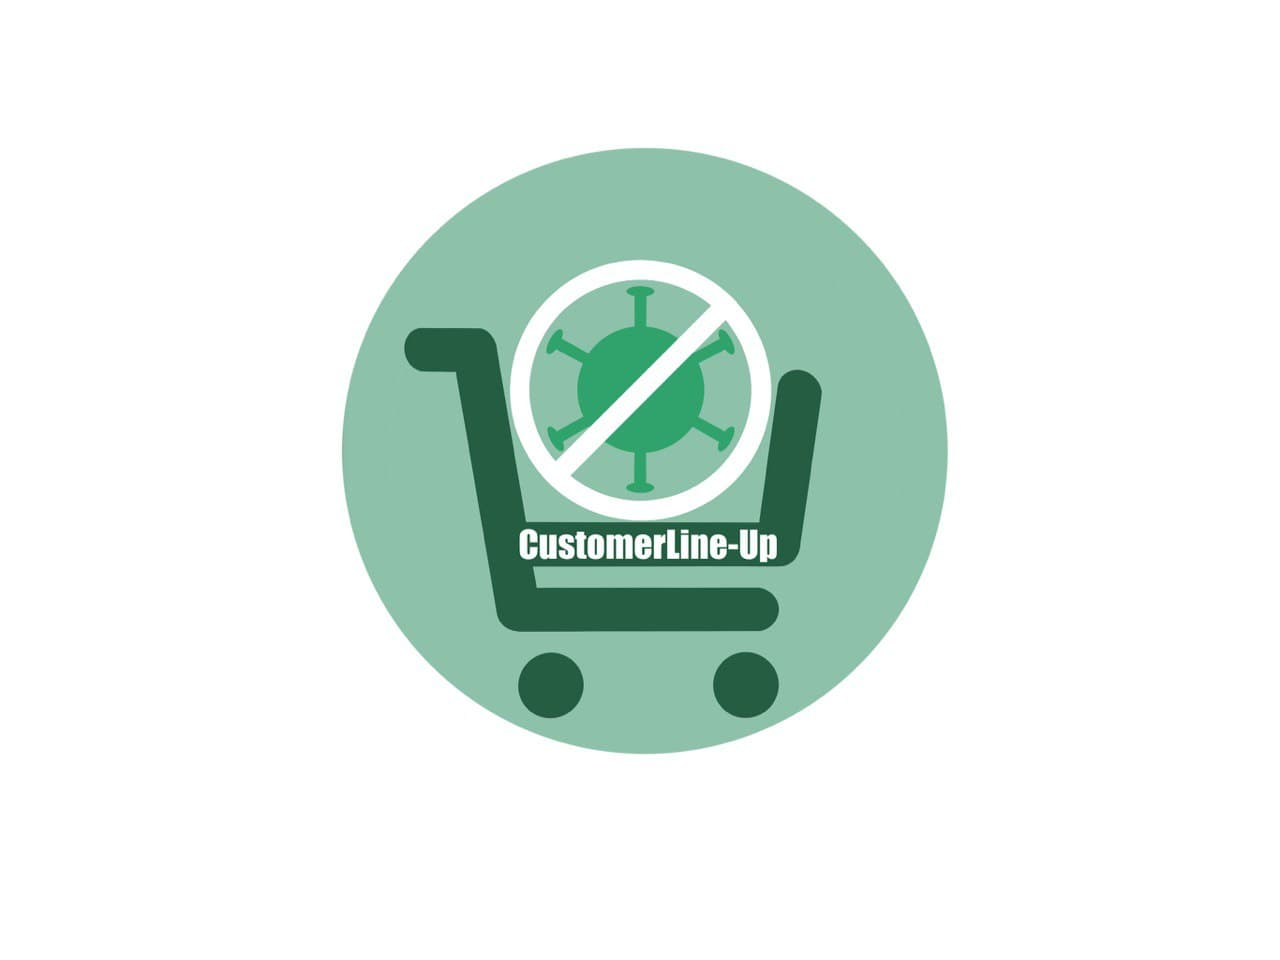
\includegraphics[scale=0.25]{img/logo.jpg}
\end{figure}
\end{center}
\vspace*{\fill}
\end{titlepage}

\normalsize


\newpage
\tableofcontents
\newpage

\section{Introduction}
\subsection{Purpose}
After showing a general description of the CL-up application within the RASD, this document focuses on analyzing the system's architecture and design, in order to satisfy the various requirements stated in the previous document. The purpose of the document is to provide a functional description of the main architectural components, showing their runtime behaviour and interactions and their interfaces. This document is mainly intended to be used by the developers and testers.

\subsection{Scope}
Customer Line-up (CL-up) is an application that aims to allow accesses to Stores in a safe way. The objective is to avoid as much as possible queue formation outside the Stores and limits the number of people inside it in an efficient way. To pursue this goal, the application allows Users to register either as a Managers or Customers, providing services to both of them. Managers can create their Stores within the app and allow other Managers to help them in the organization of the Store rules. Tools are provided to allow Customers to book Visits or Tickets to the Stores remotely, allowing a greater and more efficient way for maintaining social distancing. This is done by the use of a virtual queue managed by the System, in which Customers' Reservations are stored and managed. In order to organize the various entrances in the Stores, an identifier for each Consumer will be used, that is a QRCode.\\ %The application provides also a fall-back option (Paper Tickets) and suggestions for Customers.
\\
More information can be found in the Chapter 1 of the RASD.

\end{document}
